\section{Introduction}\label{intro}
Statistical models trained on historical data facilitate several important predictive applications such as fraud detection, recommendation systems, and automatic content classification.
In a survey of Apache Spark users, over 60\% responded that support for advanced statistical analytics was Spark's most important feature~\cite{sparksurvey}.
This sentiment is echoed across both industry and academia, and there has been significant interest in improving the efficiency of model training pipelines~\cite{bdas, alexandrov2014stratosphere, crotty2014tupleware, tensor}. 
Although it is often overlooked, an important step in all model training pipelines is handling dirty or inconsistent data including extracting structure, imputing missing values, and handling incorrect data.
Analysts widely report that cleaning dirty data is a major concern~\cite{kandel2012,nytimes}, and consequently, it is important to understand the efficiency and correctness of such operations in the context of emerging statistical analytics.

While many aspects of the data cleaning problem have been well-studied for SQL analytics, the results can be counter-intuitive in high-dimensional statistical models.
For example, studies have shown that many analysts do not approach cleaning as a one-shot pre-processing step, and instead, repeatedly alternate between cleaning and analysis.
It is common to use the preliminary analysis on dirty data as a guide to help identify potential errors and design repairs~\cite{kandel2012}.
Unfortunately, for statistical models, iteratively cleaning some data and re-training on a partially clean dataset can lead to biases in even the simplest models.

Consider a linear regression model on systematically translated data (Figure \ref{update-arch1}a).
If one only cleans two of the data points, the intermediate result reveals a misleading trend (Figure \ref{update-arch1}b).
This is a consequence of the well-known Simpson's paradox where aggregates over different populations of data can result in spurious relationships~\cite{simpson1951interpretation}. 
Similarly, statistical models face more dramatic sampling effects than the traditional 1D  \sumfunc, \countfunc, \avgfunc SQL aggregates (Figure \ref{update-arch1}c).
The challenges with Simpson's paradox and sampling are problematic because recent advances in SQL data cleaning, such as Sample-and-Clean~\cite{wang1999sample} and Progressive Data Cleaning~\cite{altowim2014progressive, papenbrock2015progressive, DBLP:journals/pvldb/YakoutENOI11}, actually advocate cleaning subsets of data to avoid the potentially expensive cleaning costs.
Clearly, such data cleaning approaches will have to be re-evaluated for the statistical modeling setting, and this paper explores how to adapt such approaches with guarantees of convergence for an important class of modeling problems. 

Data cleaning is a broad problem that encompasses extraction, de-duplication, schema matching, and many other problems in relational data.
We focus on two common operations that often require iterative cleaning, removing outliers and attribute transformation.
For example, battery-powered sensors can transmit inaccurate measurements when battery levels are low \cite{DBLP:conf/pervasive/JefferyAFHW06}. 
Similarly, data entered by humans can be susceptible to a variety of inconsistencies (e.g., typos), and unintentional cognitive biases~\cite{DBLP:conf/recsys/KrishnanPFG14}.
Since these two types of errors do not affect the schema or leave any obvious signs of corruption (e.g., NULL values), model training may seemingly succeed--albeit with an inaccurate result.

\begin{figure}[t]
\centering
 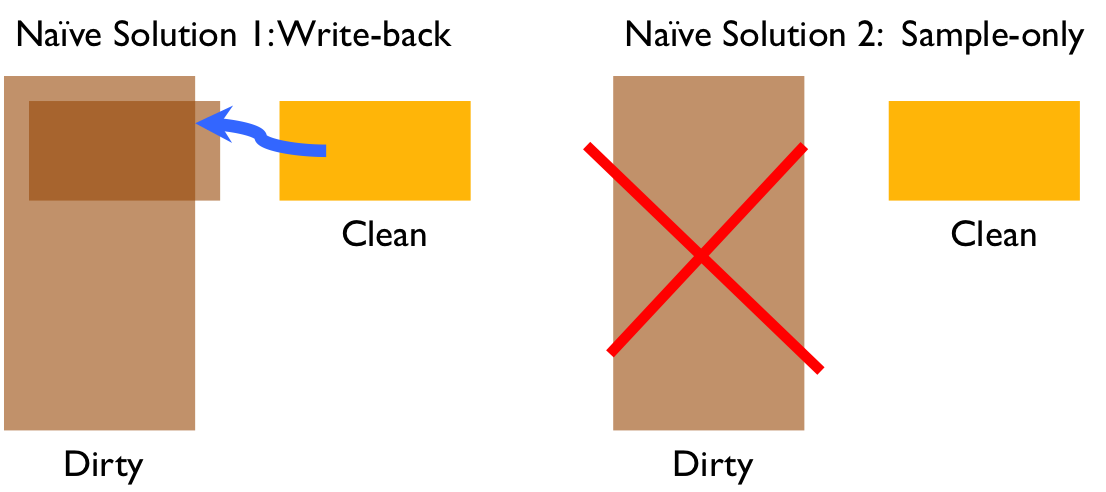
\includegraphics[width=\columnwidth]{figs/update-arch.png}
 \caption{(a) Systematic corruption in one variable can lead to a shifted model. 
 (b) Mixed dirty and clean data results in a less accurate model than no cleaning.
(c) Small samples of only clean data can result in similarly inaccurate models. \label{update-arch1}}
\vspace{-2em}
\end{figure}

We propose \sys, a model training framework that allows for iterative data cleaning while preserving provable convergence properties.
The analyst initializes \sys with a model, a featurization function, and a pointer to a dirty relational table.
In each iteration, \sys suggests a sample of data to clean based on the value to the model and the likelihood that it is actually dirty.
The analyst can apply value transformations and filtering operations to the sample. 
\sys will incrementally and safely update the current model (as opposed to complete re-training).
We propose several novel optimizations that leverage information from the model to guide data cleaning towards the records most likely to be dirty and most likely to affect the results.
%\sys can also incorporate prior knowledge about records that are likely to be dirty.

From a statistical perspective, our key insight is to treat the cleaning-training iteration as a form of Stochastic Gradient Descent, an iterative optimization method.
We treat the dirty model as an initialization, and incrementally take gradient steps (cleaning a sample of records) towards the global solution (i.e., the clean model).
Our argument ensures global convergence with a provable rate for an important class of models called \emph{convex}-loss models which include SVMs, Linear Regression, and Logistic Regression.
Convexity is a property that ensures that the iterative optimization converges to a true global optimum, and we can apply convergence arguments from convex optimization theory to show that \sys converges.

This paper describes the entire \sys architecture. However, the correctness of many of the components require detailed statistical proofs, which we have included in our extended technical report~\cite{activecleanarxiv}. To summarize our contributions:
\begin{itemize}[noitemsep]
\item We propose \sys, which allows for progressive data cleaning and statistical model training with guarantees.
\item \textbf{Correctness} We show how to update a dirty model given newly cleaned data. This update converges monotonically in expectation with a with rate $O(\frac{1}{\sqrt{T}})$.
\item \textbf{Optimizations} We derive a theoretically optimal sampling distribution that minimizes the update error and an approximation to estimate the theoretical optimum. We further show that \sys can integrate with existing dirty data detection techniques. Our proposed optimizations can improve model accuracy by up-to 2.5x for the same amount of data cleaned.
\item \textbf{Experiments} The experiments evaluate these components on five datasets with real and synthetic corruption. In a fraud prediction example, \sys examines nearly 10x less records than alternatives to achieve an 80\% true positive rate.
\end{itemize}






